\documentclass{beamer}

\usepackage[T2A]{fontenc}
\usepackage[utf8]{inputenc}
\usepackage[english,russian]{babel}
\input{settings.tex}

\newcommand{\degree}{^{\circ}}     



\title{АЧХ, ФЧХ, Боде, Найквист}
\subtitle{Теория Управления, лекция 5}
\author{Сергей Савин}
\centering
\date{\mydate}



\begin{document}
\maketitle



\begin{frame}{Входной синусоидальный сигнал}
	\begin{flushleft}
		
		Рассмотрим синусоиду с фазовым сдвигом. Её можно представить в двух формах:
		
		\begin{align}
			u(t) &= A \sin (\omega t) + B \cos (\omega t) = \\
			&= M \sin  (\omega t + \varphi)
		\end{align}
		
		где $M = \sqrt{A^2 + B^2}$ — амплитуда сигнала, а $ \varphi = - \tan^{-1} \left( \frac{B}{A} \right)$ — фазовый сдвиг.
		
		\bigskip
		
		Рассмотрим преобразования Лапласа:
		%
		\begin{align}
			\mathcal{L} (\sin (\omega t)) &= \frac{\omega}{s^2 + \omega^2}
			\\
			\mathcal{L} (\cos (\omega t)) &= \frac{s}{s^2 + \omega^2}
			\\
			\mathcal{L} (A \sin (\omega t) + B \cos (\omega t) ) &= \frac{A \omega + B s}{s^2 + \omega^2}
		\end{align}		
		
	\end{flushleft}
\end{frame}

\begin{frame}{ОДУ с входным синусоидальным сигналом}
	\begin{flushleft}
		
		Дано ОДУ с синусоидальным входным воздействием:
		
		\begin{align}
			&a_n y^{(n)} + ... + a_1 \dot y  + a_0 y = b_m u^{(m )}+ ... + b_1 \dot u + b_0 u
			\\
			&u(t) = A \sin (\omega t) 
		\end{align}
		%
		можно найти его преобразование Лапласа:
		
		\begin{align}
			&(a_n s^n + ... + a_1 s  + a_0) Y(s) = (b_m s^m + ... + b_1 s  + b_0) U(s)
			\\
			&U(s) = \frac{A \omega }{s^2 + \omega^2} 
		\end{align}
		
		таким образом:
		
		\begin{align}
			&Y(s) = \frac{b_m s^m + ... + b_1 s  + b_0}{a_n s^n + ... + a_1 s  + a_0} \cdot \frac{A \omega}{s^2 + \omega^2} 
		\end{align}
		
	\end{flushleft}
\end{frame}

\begin{frame}{Частотная характеристика}
	\begin{flushleft}
		
		\begin{block}{Частотная характеристика}
			Частотная характеристика — это установившийся выход системы при подаче на вход синусоидального сигнала.
		\end{block}
		
		\bigskip
		
		Рассмотрим систему $Y(s) = G(s)U(s)$. 
		
		\bigskip
		
		Синусоидальный входной сигнал $u(t) = A \text{sin}(\omega t)$ во временной области преобразуется в $U(s) = A \frac{\omega}{\omega^2 + s^2}$ в области Лапласа. Таким образом, при синусоидальном входном сигнале система описывается уравнением:
		
		\begin{equation}
			Y(s) = G(s)\frac{A \omega}{\omega^2 + s^2}
		\end{equation}
		
	\end{flushleft}
\end{frame}



\begin{frame}{Разложение на дроби, 1}
	\begin{flushleft}
		
		Предполагая отрицательные вещественные неповторяющиеся полюса, мы можем разложить функцию $Y(s) = G(s)\frac{A \omega}{\omega^2 + s^2}$:
		
		\begin{equation*}
			G(s)\frac{A \omega}{\omega^2 + s^2} = \frac{r_1}{s + p_1} + \frac{r_2}{s + p_2} + ... + \frac{r_n}{s + p_n} + \frac{\alpha}{s + j\omega} + \frac{\beta}{s - j\omega}
		\end{equation*}		
		
		Функция Лапласа вида $\frac{r_i}{s + p_i}$ соответствует следующей временной функции:
		
		\begin{align}
			y(t) = r_i e^{-p_i t}
		\end{align} 
		
		Таким образом, для устойчивой передаточной функции $G(s)$ при стремлении времени к бесконечности $r_i e^{-p_i t}$ стремится к нулю. Единственными компонентами функции $Y(s)$, которые не исчезают, являются последние две: $\frac{\alpha}{s + j\omega} + \frac{\beta}{s - j\omega}$.
		
	\end{flushleft}
\end{frame}


\begin{frame}{Разложение на дроби, 2}
	\begin{flushleft}
		
		Чтобы найти $\alpha$, умножим уравнение на $s + j\omega$:
		
		\begin{align*}
			&G(s)\frac{A \omega \cancel{(s + j\omega)}}{ \cancel{(s + j\omega)}(s - j\omega)} 
			= \\
			&=
			\left( \frac{r_1}{s + p_1} + ... + \frac{r_n}{s + p_n} \right) 
			\textcolor{myred}{(s + j\omega) }
			+ 
			\alpha \frac{\cancel{(s + j\omega)}}{ \cancel{(s + j\omega)}}  + \frac{\beta \textcolor{myred}{(s + j\omega) }}{s - j\omega}
		\end{align*}		
		
		Полагая $s = -j\omega$, получаем:
		%
		\begin{align}
			\alpha = G(-j\omega)\frac{A }{-2j} 
		\end{align}
		
		Чтобы найти $\beta$, умножим уравнение разложения на $s - j\omega$ и затем положим $s = j\omega$:
		%
		\begin{align}
			\beta = G(j\omega)\frac{A}{2j} 
		\end{align}
		
	\end{flushleft}
\end{frame}


\begin{frame}{Обратное преобразование Лапласа}
	\begin{flushleft}
		
		Лапласов образ установившегося решения имеет вид:
		
		\begin{align}
			Y_{ss}(s) &= \frac{\alpha}{s + j\omega} + \frac{\beta}{s - j\omega} =
			\\
			&=
			\frac{A}{2j}
			\left(
			G(j\omega)\frac{1}{s - j\omega} -G(-j\omega) \frac{1}{s + j\omega}
			\right)
		\end{align}
		
		Обратное преобразование Лапласа даёт нам:
		
		\begin{align}
			y_{ss}(t) &= 
			\frac{A}{2j}
			\left(
			G(j\omega)e^{ j\omega t} - G(-j\omega) e^{- j\omega t}
			\right)
		\end{align}
		
	\end{flushleft}
\end{frame}



\begin{frame}{Функция комплексной переменной}
	\begin{flushleft}
		
		Комплексную функцию $W(x)$ можно представить в полярной форме:
		%
		\begin{align}
			W(x) = r(x) e^{\theta(x) i}
		\end{align}
		%
		где 
		%
		\begin{align}
			r(x) &= |W(x)| = \text{амплитуда}(W(x))
			\\
			\theta(x) &= \text{фаза}(W(x)) = \text{atan2}( \text{Im}(W(x)), \ \text{Re}(W(x))  )
		\end{align}
		
		Мы наблюдаем следующие свойства комплексной сопряженности:
		%
		\begin{align}
			|W(jx)| &= |W(-jx)|
			\\
			\text{фаза}(W(-jx)) &= -\text{фаза}(W(jx))
		\end{align}
		
		\bigskip
		
		Представим синусоидальную функцию как разность:
		%
		\begin{align}
			\sin(x) = \frac{e^{jx}-e^{-jx}}{2j}
		\end{align}
		
	\end{flushleft}
\end{frame}


\begin{frame}{Амплитуда и фаза, 1}
	\begin{flushleft}
		
		Мы можем ввести представление в полярных координатах:
		
		\begin{align}
			G(j\omega) = r(\omega) e^{\theta(\omega) j} 
			\\
			G(-j\omega) = r(\omega) e^{-\theta(\omega) j}
		\end{align}
		%
		где $r(\omega) = |G(j\omega)|$ и 
		$\theta(\omega) = \text{atan2}( \text{Im}(G(j\omega)), \ \text{Re}(G(j\omega))  )$.
		
		\bigskip
		
		Мы можем переписать установившееся решение $y_{ss}(t) = 
		\frac{A}{2j}
		\left(
		G(j\omega)e^{ j\omega t} - G(-j\omega) e^{- j\omega t}
		\right)$ как:
		
		\begin{align}
			y_{ss}(t) &= 
			\frac{A}{2j}
			\left(
			r(\omega) e^{j \theta(\omega) }e^{ j\omega t} - r(\omega) e^{-j\theta(\omega) } e^{- j\omega t}
			\right)
			\\
			y_{ss}(t) &= 
			\frac{A r(\omega)}{2j}
			\left(
			e^{j \theta(\omega) + j\omega t} - e^{-(j \theta(\omega) + j\omega t)}
			\right)
			\\
			y_{ss}(t) &= 
			A r(\omega) \sin (\omega t + \theta(\omega))
		\end{align}
		
	\end{flushleft}
\end{frame}


\begin{frame}{Амплитуда и фаза, 2}
	\begin{flushleft}
		
		Таким образом, мы нашли установившийся выход системы:
		
		\begin{align}
			y_{ss}(t) &= 
			A r(\omega) \sin (\omega t + \theta(\omega))
		\end{align}
		
		Найдем отношение амплитуды выхода к амплитуде входа:
		
		\begin{align}
			\text{коэффициент усиления}(\omega)
			=
			\frac{A r(\omega)}{A} = r(\omega) = |G(j\omega)|
		\end{align}
		
		Найдем фазовый сдвиг между входным и выходным сигналами:
		
		\begin{align}
			\text{фаза}(\omega)
			=
			\theta(\omega) 
			=
			\angle G(j\omega)
			%\text{atan2}( \text{Im}(G(j\omega)), \ \text{Re}(G(j\omega))  )
		\end{align}
		
	\end{flushleft}
\end{frame}




\begin{frame}{Диаграмма Боде}
	\begin{flushleft}
		
		Первая ключевая идея диаграммы Боде заключается в подстановке чисто комплексной переменной $j \omega$ вместо переменной Лапласа $s$.
		
		\bigskip
		
		Для заданной передаточной функции $W(s)$, где $s = \sigma + j \omega$, мы можем проанализировать её поведение при $\sigma = 0$. Мы можем построить:
		
		\begin{itemize}
			\item амплитудно-частотную характеристику (АЧХ) $a(\omega) = \left| W(j \omega) \right|$,
			
			\item фазо-частотную характеристику (ФЧХ) $\varphi(\omega) = \angle W(j\omega)$.
		\end{itemize}
		
		\bigskip
		
		Диаграмма Боде представляет собой два графика: 
		
		\begin{enumerate}
			\item  $20 \cdot \text{log}_{10}\left| W(j \omega) \right|$ (логарифмическая АЧХ),
			
			\item $\frac{180}{\pi} \angle W(j\omega)$ (логарифмическая ФЧХ).
		\end{enumerate}
		
		Коэффициент 20 и логарифм связаны с тем, что вертикальная ось представлена в децибелах. 
		
	\end{flushleft}
\end{frame}

\begin{frame}{Диаграмма Боде - пример}
	\begin{flushleft}
		
		Рассмотрим $W(s) = \frac{1}{1 + s}$. Тогда $W(j \omega) = \frac{1}{1 + j \omega}$. Диаграмма Боде определяется как:
		
		\begin{align}
			\text{АЧХ:}& \ \ 
			\left|  \frac{1}{1 + j \omega} \right| =  \frac{1}{|1 + j \omega|} = 
			\frac{1}{\sqrt{1 + \omega^2}}
			\\
			\text{ФЧХ:}& \ \ 
			\angle \frac{1}{1 + j \omega} = \angle 1 - \angle (1 + j \omega) = \\ &= 0 - \tan^{-1} \left( \frac{\omega}{1} \right) = -\tan^{-1}(\omega)
		\end{align}
		
	\end{flushleft}
\end{frame}

\begin{frame}{Диаграмма Боде - запасы устойчивости}
	\begin{flushleft}
		
		{\small
		Прежде чем обсуждать применение диаграммы Боде, напомним, что передаточная функция замкнутой системы имеет вид:
		
		\begin{equation}
			W(s) = \frac{H(s)G(s)}{1 + H(s)G(s)}
		\end{equation}
		
		Определяя \emph{разомкнутую} передаточную функцию $L(s) = H(s)G(s)$, получаем:
		
		\begin{equation}
			W(j\omega) = \frac{L(j \omega)}{1 + L(j \omega)}
		\end{equation}
		
		Отсюда видно, что $W(\omega)$ становится неограниченной при $L(j \omega) = -1$. Это означает, что мы хотим избежать одновременного выполнения двух условий: равенства модуля $|L(j \omega)|$ единице и равенства его фазы (аргумента) $180\degree$ (напомним, фаза $0\degree$ соответствует чисто положительному действительному числу, фаза $90\degree$ — чисто положительному мнимому числу, $180\degree$ — чисто отрицательному действительному числу и т.д.).
		
		}
		
	\end{flushleft}
\end{frame}


\begin{frame}{Запасы устойчивости - пример}
	
	% credit: https://www.electrical4u.com/bode-plot-gain-margin-phase-margin/
	\begin{figure}
		\centering
		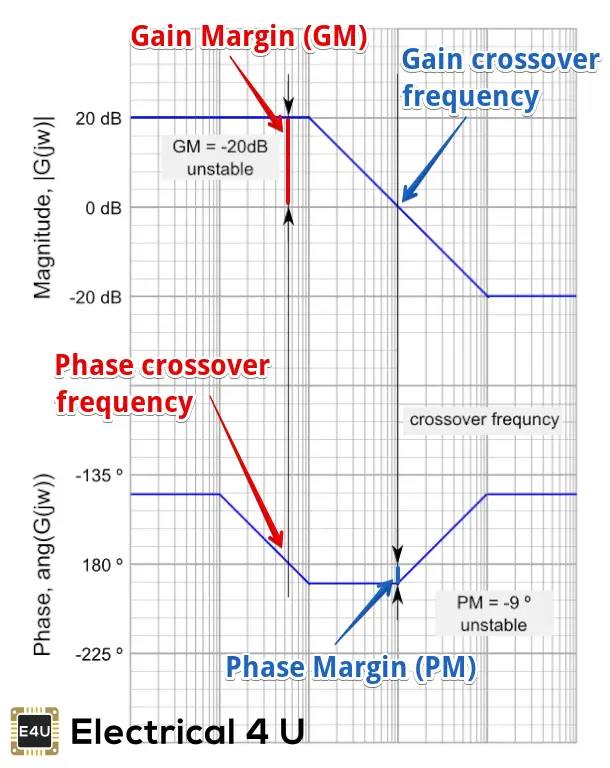
\includegraphics[width=0.68\linewidth]{bode-plot}
		\caption{Иллюстрация запасов устойчивости на диаграмме Боде}
		\label{fig:bode-plot}
	\end{figure}
	
	
\end{frame}

\begin{frame}{Диаграмма Боде с резонансом, 1}
	\begin{flushleft}
		
		Рассмотрим систему с резонансом:
		%
		\begin{equation}
			\begin{cases}
				\dot{\bo{x}} = 
				\begin{bmatrix}
					0 & 1 \\
					-1 & 0
				\end{bmatrix}
				\bo{x}
				+ 
				\begin{bmatrix}
					0\\
					1
				\end{bmatrix}
				\bo{u} 
				\\
				\bo{y} = 
				\begin{bmatrix}
					1 & 0
				\end{bmatrix}
				\bo{x}
			\end{cases}
		\end{equation}
		
		
		Амплитудно-частотная характеристика для этой системы равна $\frac{1}{|1-\omega^2|}$.
		
		\bigskip
		
		Матрица состояния этой системы имеет собственные значения $\lambda_i = \pm j$, резонансная частота $\omega = 1$.
		
	\end{flushleft}
\end{frame}

\begin{frame}{Диаграмма Боде с резонансом, 2}
	
	% credit: https://www.electrical4u.com/bode-plot-gain-margin-phase-margin/
	\begin{figure}
		\centering
		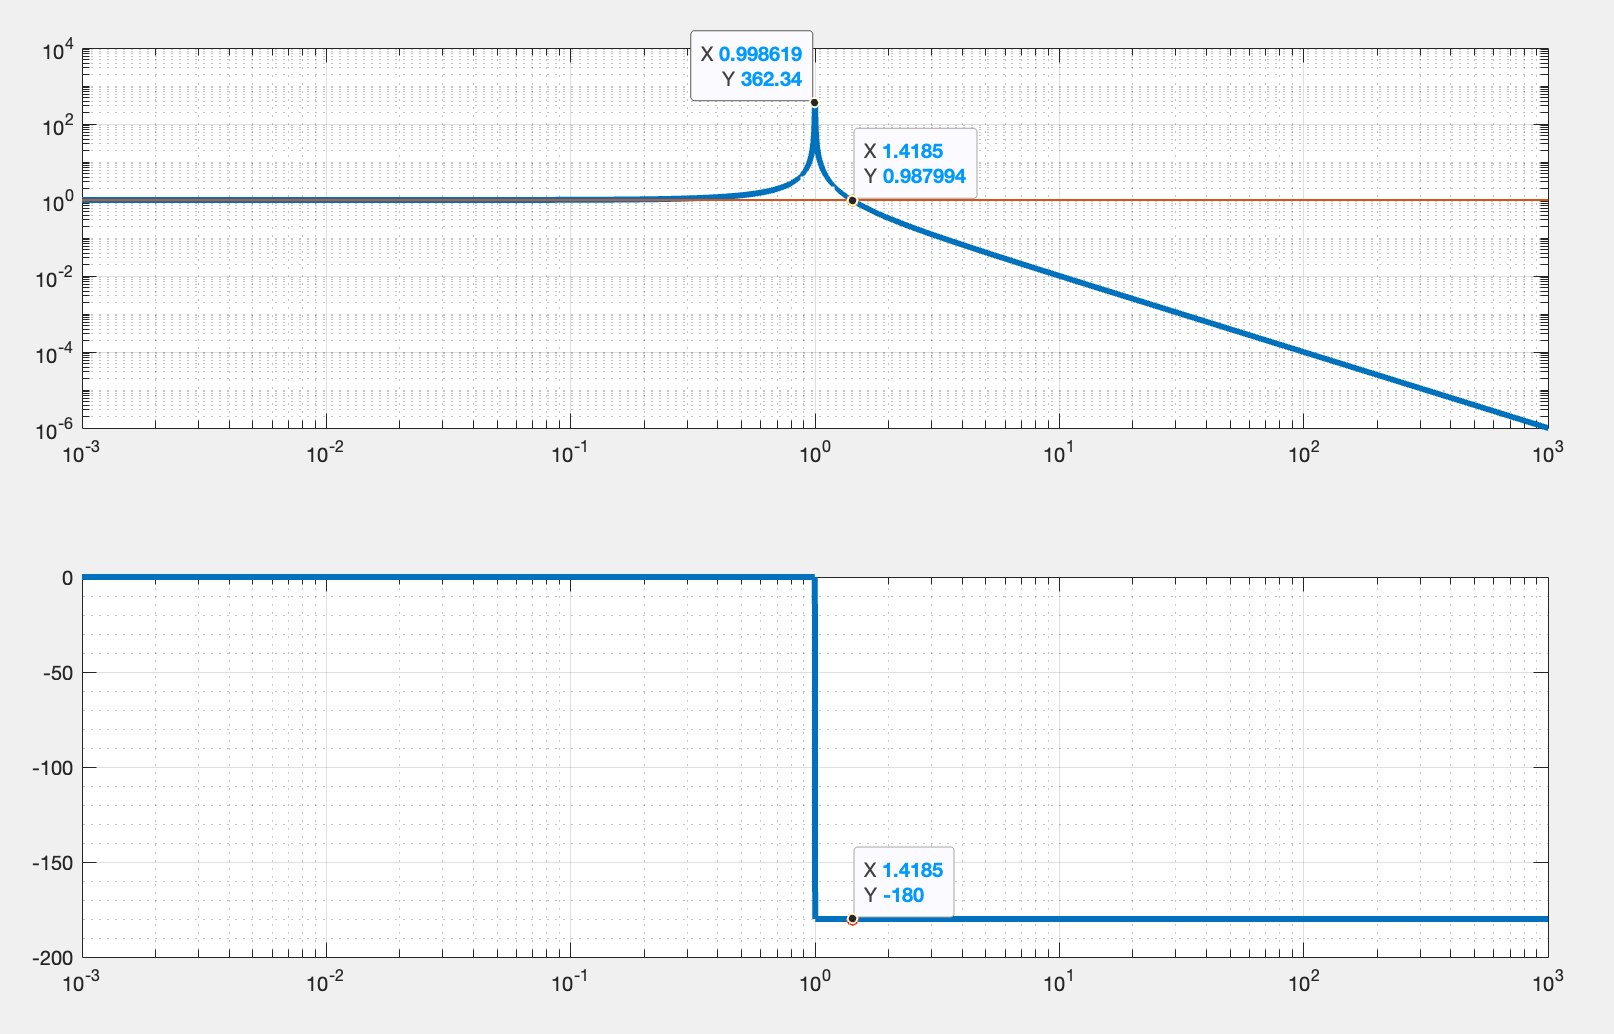
\includegraphics[width=0.8\linewidth]{Resonance}
		\caption{Диаграмма Боде системы с резонансом}
		\label{fig:Resonance}
	\end{figure}
	
	\begin{flushleft}
		\small
		\textit{Примечание:} На резонансной частоте $\omega = 1$ наблюдается резкий пик амплитуды (теоретически стремящийся к бесконечности) и скачкообразное изменение фазы на $-180\degree$.
	\end{flushleft}
	
\end{frame}

\begin{frame}{Диаграмма Найквиста}
	\begin{flushleft}
		
		\emph{Диаграмма Найквиста} (годограф Найквиста) для передаточной функции $L(s)$ — это график $L(j\omega)$, построенный для $\omega \in (-\infty, \  \infty )$ на комплексной плоскости.
		
		\bigskip
		
		Как обсуждалось ранее, передаточная функция замкнутой системы становится неограниченной при значении разомкнутой передаточной функции $L(s) = -1$. Для диаграммы Найквиста: 
		
		\begin{itemize}
			\item запас по фазе — это угол, на который можно повернуть график до его пересечения с точкой -1;
			
			\item запас по амплитуде — это масштабирование (растяжение/сжатие) графика до его пересечения с точкой -1.
		\end{itemize}
		
		Однако, с помощью диаграммы Найквиста мы можем непосредственно видеть расстояние между графиком и точкой -1 \textbf{по обеим координатам} одновременно.
		
	\end{flushleft}
\end{frame}

\begin{frame}{Пример диаграммы Найквиста}
	
	% TODO: \usepackage{graphicx} required
	\begin{figure}
		\centering
		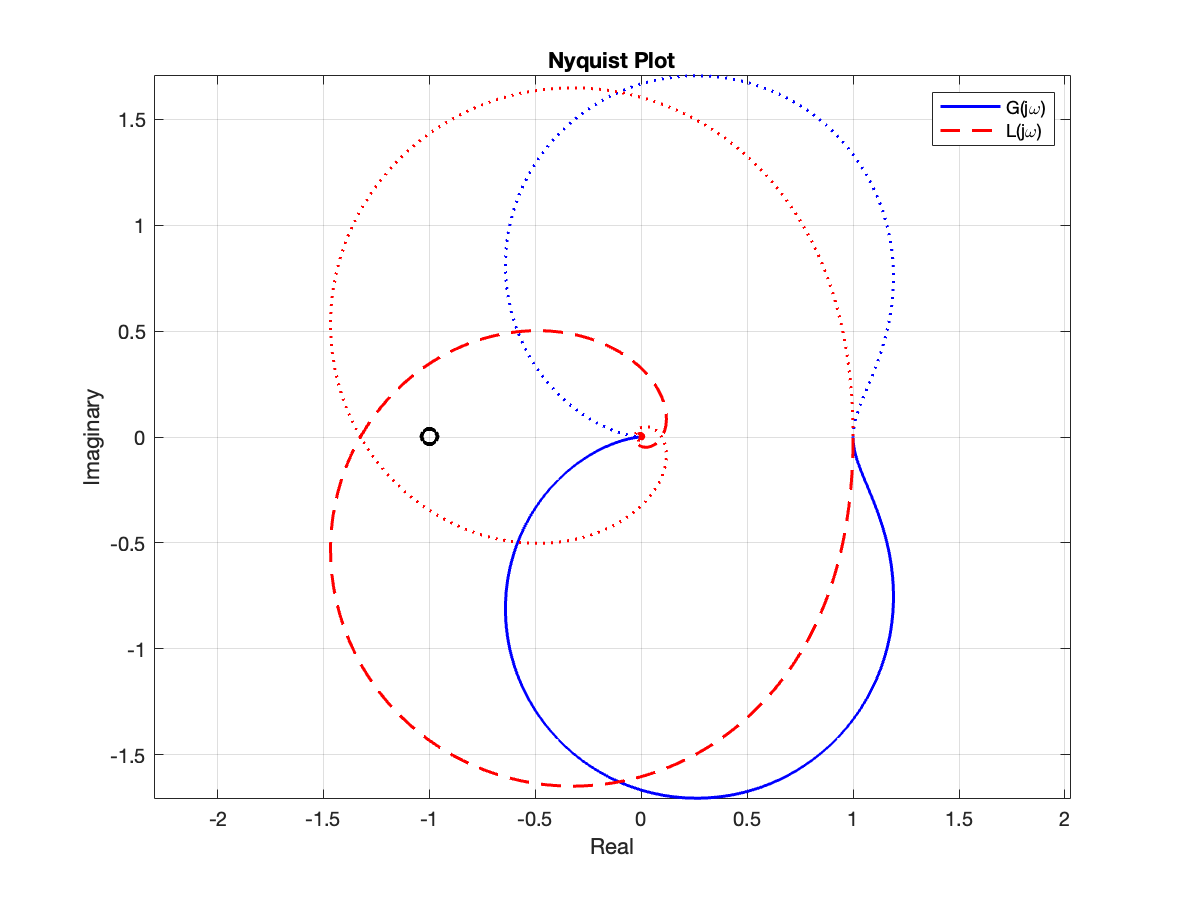
\includegraphics[width=0.8\linewidth]{Nyquist}
		\caption{Диаграмма Найквиста}
		\label{fig:nyquist}
	\end{figure}

	
\end{frame}

\begin{frame}{Диаграмма Боде для той же системы}
	
	% TODO: \usepackage{graphicx} required
	\begin{figure}
		\centering
		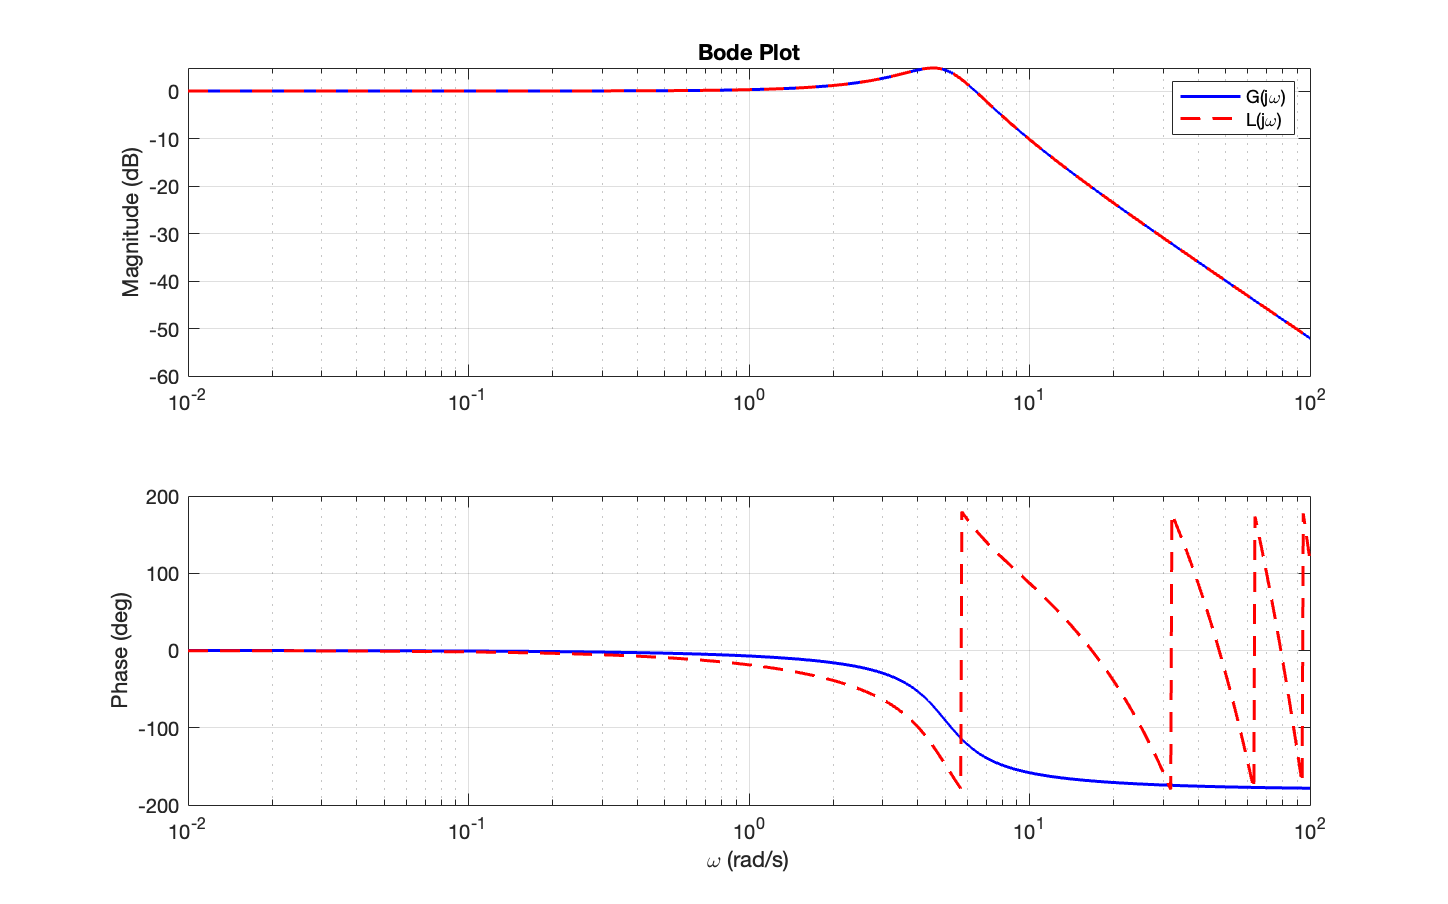
\includegraphics[width=0.9\linewidth]{Bode}
		\caption{Диаграмма Боде для той же системы, что и на предыдущем слайде}
		\label{fig:bode}
	\end{figure}
	
	
\end{frame}


\begin{frame}{Литература}

\begin{itemize}
	
	
\item Nise, N.S. Control systems engineering. John Wiley \& Sons. (Chapter 10 Frequency Response Techniques)	
	

\item \bref{https://control.asu.edu/Classes/MAE318/318Lecture18.pdf}{Matthew M. Peet; Systems Analysis and Control - Lecture 18: The Frequency Response}	
	
	
\item \bref{https://youtu.be/_eh1conN6YM}{Control System Lectures - Bode Plots, Introduction}

\item \bref{https://global.oup.com/us/companion.websites/fdscontent/uscompanion/us/static/companion.websites/9780199339136/Appendices/Appendix_F.pdf}{Oxford University Press. s-Domain analysis: poles, zeros, and Bode plots}


\end{itemize}

\end{frame}




\myqrframe



\begin{frame}{Преобразования Лапласа и Фурье}
	\begin{flushleft}
		
		\begin{itemize}
			\item \emph{Ряд Фурье} можно рассматривать как представление периодической функции в виде суммы гармоник (синусов и косинусов). Эти синусы и косинусы можно считать образующими базис в линейном пространстве. Коэффициенты ряда можно рассматривать как дискретный спектр функции.
			
			\item \emph{Преобразование Фурье} дает непрерывный спектр функции. "Базис" образован синусоидальными и косинусоидальными функциями всех частот (непрерывная суперпозиция комплексных экспонент $e^{j \omega t}$).
			
			\item \emph{Преобразование Лапласа} также дает непрерывный спектр, но в базисе, образованном комплексными экспонентами. Мне нравится представлять этот базис как решения дифференциальных уравнений второго порядка.
		\end{itemize}
		
	\end{flushleft}
\end{frame}

\begin{frame}{Преобразования Лапласа и Фурье}
	\begin{flushleft}
		
		Давайте сравним. Преобразование Фурье:
		
		\begin{equation}
			F(\omega) = \int_{-\infty}^\infty f(t) e^{-j t \omega} dt, \ \ \omega \in \mathbb{R}
		\end{equation}
		
		Преобразование Лапласа:
		
		\begin{equation}
			F(s) = \int_0^\infty f(t) e^{-st}dt, \ \ s \in \mathbb{C}
		\end{equation}
		
		Можно заметить, что преобразование Фурье похоже на преобразование Лапласа с чисто мнимым числом в показателе степени.
		
	\end{flushleft}
\end{frame}

\begin{frame}{Преобразование Лапласа и установившееся решение}
	\begin{flushleft}
		
		Из анализа решений линейных ОДУ мы знаем, что при гармоническом входном сигнале (синус, косинус или их комбинация) "после завершения переходного процесса решение стремится к гармонической функции той же частоты", но с возможным изменением амплитуды и фазы.
		
		\bigskip
		
		Интуитивно можно считать, что мнимая часть переменной $s$ связана с колебаниями, а действительная часть — с затуханием/ростом. 
		
		\bigskip
		Ядро преобразования Лапласа — это функция $e^{-st}$, где $s = \sigma + j \omega$ — комплексная переменная. Если $\sigma = 0$, ядро принимает вид $e^{-j \omega t} = \text{cos}(\omega t) - j \text{sin}(\omega t)$. Здесь можно увидеть сходство с ядром преобразования Фурье.
		
	\end{flushleft}
\end{frame}




\end{document}
